
\documentclass[tikz, border=1mm]{standalone}

\usepackage{amsmath}

\usepackage{tikz}

\usetikzlibrary{calc,angles,quotes,intersections,shapes.geometric}

\usepackage{tkz-euclide}

\begin{document}

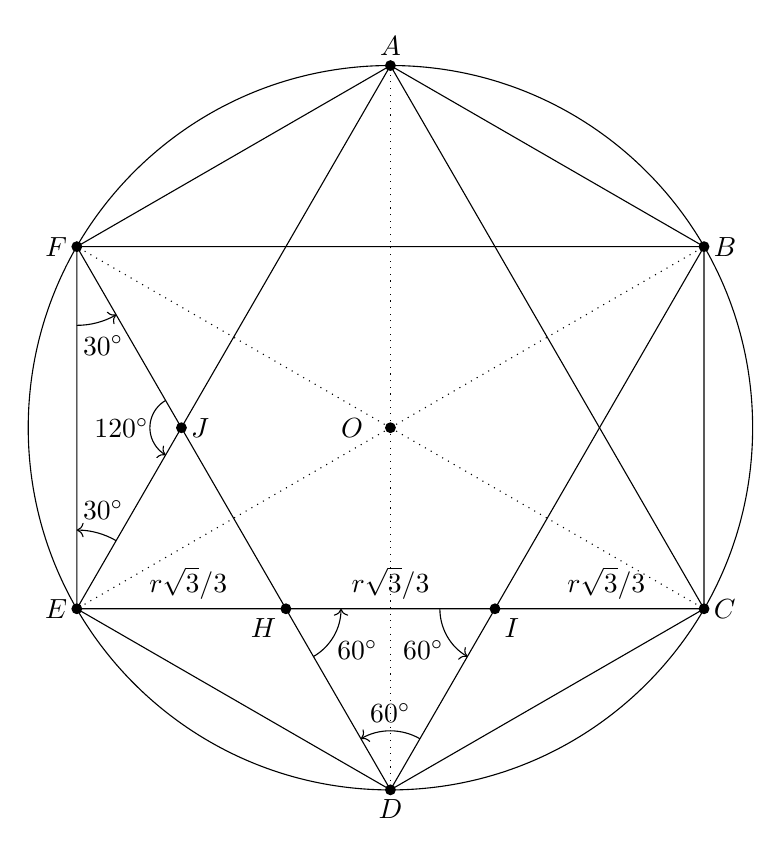
\begin{tikzpicture}[scale=2.3]

	% parameters
	\def\numsides{6}
	\def\radius{2}
	\def\rotation{90}

	% coordinates

	\coordinate (O) at (0,0);
	\foreach \i in {1,...,\numsides} {
		\coordinate (P\i) at ({360/\numsides*(\i-1)+\rotation}:\radius);
	}
	\coordinate (G) at (0,{-\radius/2});
	\coordinate (H) at ({-\radius*sqrt(3)/6},{-\radius/2});
	\coordinate (I) at ({\radius*sqrt(3)/6},{-\radius/2});

	% intersections

	%\path[name path=hexagram1] (P1) -- (P3);
	%\path[name path=hexagram2] (P2) -- (P4);
	%\path[name intersections={of=hexagram1 and hexagram2, by=J}];

	\tkzInterLL(P1,P3)(P2,P4)\tkzGetPoint{J}

	% circle
	\draw (O) circle (\radius);

	% polygon
	\draw (P1) \foreach \i in {2,...,\numsides} { -- (P\i) } -- cycle;

	% radiuses
	\foreach \i in {1,...,\numsides} { \draw[dotted] (O) -- (P\i); }

	% hexagram
	\draw (P1) -- (P3) -- (P5) -- cycle;
	\draw (P2) -- (P4) -- (P6) -- cycle;

	% thick vertices

	\fill (O) circle (0.3mm);
	%\fill (G) circle (0.3mm);
	\fill (H) circle (0.3mm);
	\fill (I) circle (0.3mm);
	\fill (J) circle (0.3mm);
	\foreach \i in {1,...,\numsides} { \fill (P\i) circle (0.3mm); }

	% vertices labels

	\node[label={[label distance=1.0mm]left:$O$}] at (O) {};
	%\node[circle, fill, inner sep=1pt,
	%label={[label distance=2mm]left:$O$}] at (O) {};

	\node[above] at (P1) {$A$};
	\node[right] at (P6) {$B$};
	\node[right] at (P5) {$C$};
	\node[below] at (P4) {$D$};
	\node[left] at (P3) {$E$};
	\node[left] at (P2) {$F$};

	%\node[above left] at (G) {$G$};
	\node[below left] at (H) {$H$};
	\node[below right] at (I) {$I$};
	\node[right] at (J) {$J$};

	\node[above] at ($(H)!0.5!(I)$) {$r \sqrt{3}/3$};
	\node[above right] at ($(P3)!0.3!(H)$) {$r \sqrt{3}/3$};
	\node[above right] at ($(I)!0.3!(P5)$) {$r \sqrt{3}/3$};

	\pic[draw, ->, "$60^\circ$", angle radius=0.7cm, angle eccentricity=1.5]
	{angle = P4--H--G};

	\pic[draw, ->, "$60^\circ$", angle radius=0.7cm, angle eccentricity=1.5]
	{angle = G--I--P4};

	\pic[draw, ->, "$60^\circ$", angle radius=0.75cm, angle eccentricity=1.3]
	{angle = I--P4--H};

	\pic[draw, ->, "$30^\circ$", angle radius=1.0cm, angle eccentricity=1.3]
	{angle = P3--P2--J};

	\pic[draw, ->, "$30^\circ$", angle radius=1.0cm, angle eccentricity=1.3]
	{angle = J--P3--P2};

	\pic[draw, ->, "$120^\circ$", angle radius=0.4cm, angle eccentricity=1.9]
	{angle = P2--J--P3};

\end{tikzpicture}

\end{document}
